\section{Introduction}

% important threads
%   -> We're an analysis paper (with synthetic and real tasks)
%   -> Focused on LCLMs

We have access to numerous growing digital \emph{corpora} of unstructured data containing valuable information, from email records and scientific literature to rapidly produced large language model (LLM) agent traces. Consequently, years of computer science effort have studied tasks involving analysis or extraction of corpus information, which we'll refer to with the blanket term \emph{corpus reasoning}. 

Commonly studied corpus reasoning tasks include search / information retrieval \citep{TREC2021, Hou2025CLERCAD}, summarization \citep{Kocisk2017TheNR}, code repository analysis \citep{Bai2024LongBenchVT}, and multi-hop question answering \citep{Yang2018HotpotQAAD}. These are often a focus of long-context language modeling (LCLM) work as reflected in popular benchmarks \cite{Yen2024HELMETHT, Bai2024LongBenchVT, Chen2026LongBenchPA}, and prior work has made great progress towards efficient systems to handle these \cite{Beltagy2020LongformerTL} \prasann{More cites, suggestions}. 

On the other hand, there are many other interesting corpus reasoning queries not captured by more commonly evaluated tasks: \emph{``What are all the contradicting claims?''} given a biology corpus, \emph{``What user interactions in the corpus from this year are most different from last year's?''} given a corpus of human AI interaction traces, or \emph{``What order did these events likely occur in?''} given miscellaneous historical documents. LCLMs are well-suited to such tasks, but such tasks haven't been the focus of LCLM work. We write this analysis paper to unify our understanding of corpus reasoning tasks.

Given the task-agnostic view of much prior work\prasannnote{I think the task-agnostic view needs more setup}, we first ask the question: \emph{Do all corpus reasoning tasks have the same architectural requirements at scale?} \prasannnote{Is this the right central question? I do think it's maybe not a question prior work has considered properly, and one that our work answers in a useful way.} Across a comprehensive set of 25 realistic and synthetic corpus reasoning tasks, we find the answer to be \emph{no}. We show a comparison between two tasks from our suite in Figure~\ref{fig:motivatingtask} as a motivating result: on a multi-hop retrieval setting, an efficient linear chunked attention approach scales similarly with context to standard quadratic attention, but on a contradiction search setting, chunked attention does much worse at longer contexts. This is concerning because efficient architectures are necessary to doing corpus reasoning at scale: quadratic attention is intractable over large corpora.

% \prasann{Paragraph kind of clarifying the vision and also that this is an analysis paper (not)} \prasann{Some things missing: CTC is a new "difficulty factor". }

% \prasann{talk about fact that prior work is task-agnostic}

% Not only are these tasks understudied, we observe that they may behave fundamentally differently (Figure~\ref{fig:motivatingtask}): using long-context-language models (LCLM), we find that \emph{on a well-studied multi-hop retrieval task}, the performance gap between a scalable chunked attention approach with $O(N)$ complexity (which we refer to as \cmc{N}, where A is for attention) and an expensive full attention \cmc{N^2} approach remains small, even as corpus size grows. On the other hand, \emph{on a less-studied task} involving searching for contradicting claims, \emph{the gap between cheap and expensive attention grows by over 3x with the same increase in context size}. This is concerning because efficient architectures are necessary to doing corpus reasoning at scale: \cmc{N^2} attention is intractable over large corpora.

Why do tasks scale so differently with corpus size? We propose a new conceptual framework---\emph{corpus task complexity} (CTC)---that allows us to, independent of methods, characterize more challenging tasks as those which require a greater complexity of basic oracle ``operations'' with respect to corpus size $N$. We use this to categorize tasks as, for example \ctc{N} (a retrieval task where an oracle would only need to check each document once to see if they're relevant to queries), \ctc{N^2} (a task looking for a certain kind of cross-document relation, like contradiction, will need to check all possible pairs).  We assemble a diverse suite of 25 existing and synthetically constructed tasks to capture a variety of settings we'd expect to cover different complexities. % We illustrate this in Figure~\ref{fig:motivatingtask}: for factoid QA, as $N$ grows to 100, we still only need 100 operations where we check \emph{``does doc i discuss Ralph Lauren?''} for each document. However, on tasks which need to check all possible document pairs, for example \emph{``What are all contradicting claims in retrieval literature?''}, this grows to 4950 operations (corresponding to number of possible pairs) to solve the task! 

\begin{figure}[t]
    \centering
    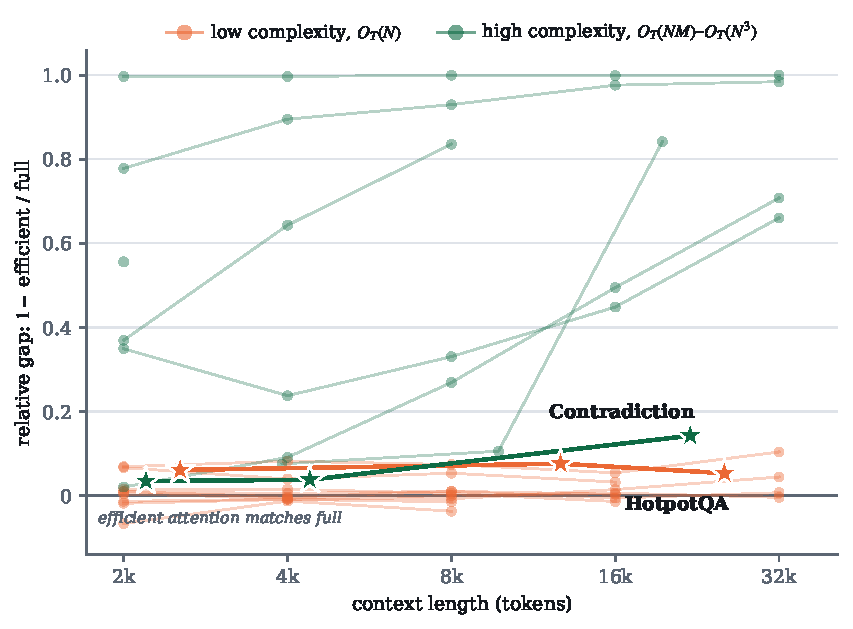
\includegraphics[width=0.72\textwidth]{figures/fig1_gap_vs_context.pdf}
    \caption{Performance gap between in-domain trained models with full and efficient attention on
    various tasks evaluated at various context lengths. \emph{Observation}: Certain tasks (in the
    orange-colored group, multi-hop retrieval highlighted) show minimal gap increase with greater
    context length, while other tasks (green-colored group, contradiction search highlighted) show
    large gap increases.}
    \label{fig:motivatingtask}
\end{figure}
\autonote{NEW figure, replacing the 4-bar \texttt{gap\_2k\_20k.pdf} (still on disk, unused) --- the
teaser you sketched in the old caption. Script: \texttt{figures/fig1\_gap\_vs\_context.py}; 65 points
over 16 tasks $+$ the two starred ladders. \textbf{Mixed sources, on purpose:} the cloud is the
CTC-suite grid (Qwen3.5-4B full-FT, full vs chunked$+$mask-mixing), but contradiction, HotpotQA and
grouping come from the earlier per-N corpus-reasoning runs --- contradiction because its suite ladder
is the suspect one (its suite gap actually \emph{shrinks}, 0.376$\to$0.302, since full attention itself
decays 0.849$\to$0.335), HotpotQA because the suite has no dense checkpoint at all (S3 distcp
incomplete, 80/128 shards), grouping on request. So the stars are 4B full-FT (contradiction) and 0.8B
LoRA (HotpotQA), neither matching the cloud's model --- that wants a sentence in the caption or a redo
on matched checkpoints. Contradiction's $n{=}20$ rung ($\sim$0.9k tokens) is dropped so the axis can
start at 2k. y is now the \emph{relative} gap $1-$chunked$/$full, on a plain linear axis. The raw difference
is bounded above by the full-attention score, which hid the trend on four high-complexity tasks
(reorder, textgroups capped from above as full attention collapses; strmatch, xabsence saturated from
below) --- on this axis reorder reads 0.37$\to$0.84. The cost is a floor rule (drop a rung when the
full arm is under 0.15, since a ratio of two near-zero numbers is noise), which removes
\texttt{helmet\_qa} and \texttt{mathmatch} entirely --- tasks that never trained, not tasks with no
gap --- and leaves \texttt{textgroups} a single point. \texttt{grouping}'s last point rides a full arm
of 0.196, only just above the floor. Dot colour is CTC class, not observed behaviour. After
dropping cycle and grouping-labeled and re-classing absence and outlier-Amazon as \ctc{N}, every
low-complexity task has $|$gap$| \leq 0.06$ at every rung and every high-complexity task is clear of
that band --- except \texttt{mathmatch}, whose arms are 0.003 vs 0.001, i.e.\ no signal rather than no
gap. Consider dropping it too.}

% Previous version of this figure block, kept for reference:
% \begin{figure}[t]
%     \centering
%     \begin{minipage}[b]{0.33\textwidth}
%         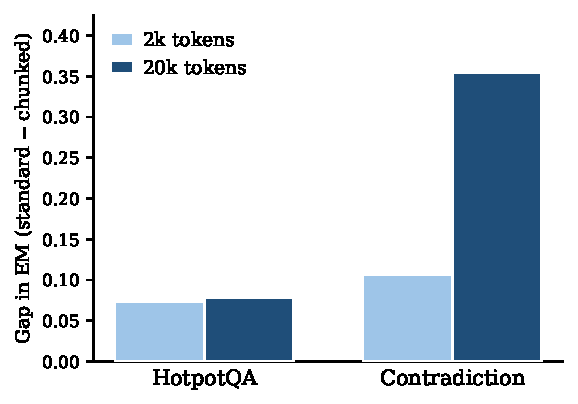
\includegraphics[width=\textwidth]{figures/gap_2k_20k.pdf}\\
%     \end{minipage}
%     \caption{\emph{Observation} (Left): At larger context lengths, the gap between expensive and cheap attention (y-axis) \textbf{widens much faster on the contradiction task compared to the factoid task} \emph{Corpus Task Complexity} \prasann{I moved half to section 2 (I felt like there was overload / it fit better there)? Left part of figure I think should have an x-axis (can maybe have some averaging or smth across tasks)} \prasann{One idea, we could give a "teaser" where we have different colors for low ctc, high-ctc, and then x-axis is context length, and y-axis is gap between efficient and standard, and then the graph will show one stays near baseline and the other increases rapidly}}
%     \label{fig:motivatingtask}
% \end{figure}



Across the large-scale corpus reasoning task suite we assemble, we find empirically that \cname greatly explains the relationship between attention-complexity and performance with larger corpus sizes. On low complexity tasks, extremely efficient and expensive standard attention approaches are largely comparable. Meanwhile, high complexity tasks consistently correspond to performance gaps emerging and growing between efficient and expensive attention methods. This is despite using Qwen-3.5, with a hybrid architecture we found most effective for chunked attention, and a new mask-mixing technique which we also empirically find to greatly improve chunked attention performance. These trends occur even at relatively small (under 32k token) context lengths, with evidence they would become even stronger at scale.

To further expand the relationship between task complexity and their computational requirements, we conduct several further analyses, finding that (a) even within attention complexity, sparser quadratic approaches may do worse than dense ones (b) much larger models with chunked attention degrade more slowly but can still scale worse on high-\cname tasks than smaller quadratic attention models\prasannnote{TODO unify quadratic, dense, chunked, etc. a bit}, and (c) increasing the difficulty of atomic operations within the task can increase these gaps (\prasann{TODO no evidence for this yet but will get soon}). \prasannnote{I feel like there's something more we can say...}

% We first investigate how LCLM \emph{learning signal} is affected by more complex settings, and investigate solutions. We find LCLM gradients to be quite sparse over context, and consequently, especially on more challenging tasks and with efficient chunked \cmc{N} inference, to face issues during training. In some settings we find faithful CoTs surprisingly effective to enable more effective and stable learning, but chunked attention still often fails to learn. We propose a new approach---mask mixing---that improves chunked inference by mixing training of standard and chunked attention.

% To determine whether our learning dynamics solutions solve the issue of more complex tasks, we then perform a larger suite of experiments at scale. The result---even with mask-mixing, the gap between chunked and standard attention grows rapidly at larger corpus sizes for understudied complex tasks like contradiction search. Our results align with our \cname framework: higher \cname tasks correspond to larger gaps between chunked and standard attention, suggesting that the computational needs of these tasks grow faster than \cmc{N} attention can keep up with. Further supporting this, we find that even smaller models with full attention can outperform larger chunked models. 

 Taken together, \textbf{our work helps identify an understudied class of \boldmath high \cname corpus reasoning tasks, and makes a case for more LCLM research to handle them at scale}. Our new task-centric perspective demonstrates that efficient methods that work for low-\cname tasks are insufficient at high-\cname, and that development of systems to handle such tasks at realistic 10M+ token scale may be a long-term open problem. Our comprehensive task suite, detailed analysis, and new methods like mask-mixing which increase train-time complexity for better inference, help provide initial paths forward. We release our task suite, code, and data to support future research in this area. 

\prasannnote{Do we need to be worried about openai graphwalks? Do we also need to be worried about efficient attention stuff like NSA and MoBA}